% ============================================================
%  SCHOLA DOMESTICA — Magister Mathematica
%  Level 1 | Week 6 | Day 2
%  Topic: Counting On and Counting Back — Number Line 0–10
%  Enrichment: Mayan numbers 6–10 (dots + bar)
% ============================================================
\documentclass[12pt, letterpaper]{article}

\usepackage[top=1in, bottom=1in, left=1in, right=1in]{geometry}
\usepackage{fontenc}
\usepackage{inputenc}
\usepackage{lmodern}
\usepackage{microtype}
\usepackage{amsmath}
\usepackage{graphicx}
\usepackage{xcolor}
\usepackage{tikz}
\usepackage{array}
\usepackage{enumitem}
\usepackage{multicol}
\usepackage{mdframed}
\usepackage{fancyhdr}

\definecolor{scholared}{RGB}{160,30,30}
\definecolor{scholagold}{RGB}{180,140,40}
\definecolor{scholacream}{RGB}{253,248,235}
\definecolor{scholagreen}{RGB}{50,110,60}
\definecolor{scholablue}{RGB}{40,80,140}
\definecolor{mayared}{RGB}{140,30,30}

\pagestyle{fancy}
\fancyhf{}
\renewcommand{\headrulewidth}{0.6pt}
\fancyhead[L]{\small\textcolor{scholared}{\textbf{Schola Domestica — Magister Mathematica}}}
\fancyhead[R]{\small\textcolor{scholared}{Level 1 · Week 6 · Day 2}}
\fancyfoot[C]{\small\textcolor{gray}{— \thepage\ —}}

\newcommand{\answerline}{\underline{\hspace{2.5cm}}}
\newcommand{\biganswerline}{\underline{\hspace{4cm}}}
\newcommand{\numbox}{\fbox{\hspace{0.6cm}\vphantom{0}}}

\newmdenv[
  backgroundcolor=scholacream,
  linecolor=scholared,
  linewidth=1.5pt,
  roundcorner=6pt,
  innertopmargin=8pt,
  innerbottommargin=8pt,
  innerleftmargin=10pt,
  innerrightmargin=10pt
]{lessonbox}

\newmdenv[
  backgroundcolor={RGB}{245,240,215},
  linecolor=mayared,
  linewidth=1.5pt,
  roundcorner=6pt,
  innertopmargin=8pt,
  innerbottommargin=8pt,
  innerleftmargin=10pt,
  innerrightmargin=10pt
]{mayanbox}

\begin{document}

\begin{center}
  {\LARGE\textbf{\textcolor{scholared}{Counting On and Counting Back}}}\\[4pt]
  {\Large\textcolor{scholagold}{\textit{Hops on the Number Line}}}\\[6pt]
  {\small Name: \biganswerline \hspace{1cm} Date: \answerline}
\end{center}

\vspace{4pt}
\noindent\textcolor{scholared}{\rule{\linewidth}{1pt}}
\vspace{4pt}

% IMAGE PROMPT (Beatrix Potter watercolour style):
% A frog leaping along a row of lily pads numbered 0 to 10 in a gentle stream.
% Each lily pad is visible, the frog is mid-jump between pad 7 and pad 9 (skipping 8).
% Soft watercolour, warm green-gold tones. No text.

\begin{lessonbox}
\textbf{Counting On} means jumping \textbf{forward} on the number line (getting bigger).\\[4pt]
\textbf{Counting Back} means jumping \textbf{backward} on the number line (getting smaller).\\[6pt]
\begin{center}
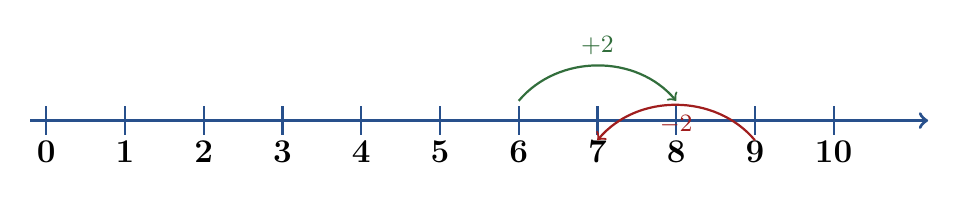
\begin{tikzpicture}[scale=1]
  \draw[very thick, scholablue, ->] (-0.2,0) -- (11.2,0);
  \foreach \n in {0,...,10} {
    \draw[thick, scholablue] (\n,0.18) -- (\n,-0.18);
    \node[below=4pt] at (\n,0) {\large\textbf{\n}};
  }
  % forward hop example: 6 -> 8
  \draw[->, thick, scholagreen, bend left=50] (6,0.25) to node[above]{\small +2} (8,0.25);
  % backward hop example: 9 -> 7
  \draw[->, thick, scholared, bend right=50] (9,-0.25) to node[below]{\small $-2$} (7,-0.25);
\end{tikzpicture}
\end{center}
\end{lessonbox}

\bigskip

% ===== PART I: COUNT ON =====
\noindent\textcolor{scholared}{\large\textbf{Part I — Count On (Forward)}} \hfill \textit{(Problems 1–5)}

\medskip

\begin{center}
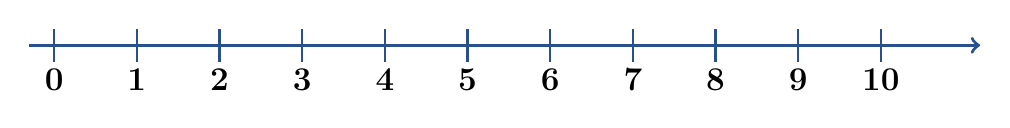
\begin{tikzpicture}[scale=1.05]
  \draw[very thick, scholablue, ->] (-0.3,0) -- (11.2,0);
  \foreach \n in {0,...,10} {
    \draw[thick, scholablue] (\n,0.2) -- (\n,-0.2);
    \node[below=5pt] at (\n,0) {\large\textbf{\n}};
  }
\end{tikzpicture}
\end{center}

\medskip
\noindent\textit{Draw the hops and write the answer. Use the number line above.}

\bigskip
\noindent\textbf{1.} Start at \textbf{6}. Count on \textbf{3}. Land on: \hfill \answerline

\bigskip
\noindent\textbf{2.} Start at \textbf{7}. Count on \textbf{2}. Land on: \hfill \answerline

\bigskip
\noindent\textbf{3.} Start at \textbf{8}. Count on \textbf{1}. Land on: \hfill \answerline

\bigskip
\noindent\textbf{4.} Start at \textbf{5}. Count on \textbf{4}. Land on: \hfill \answerline

\bigskip
\noindent\textbf{5.} Start at \textbf{6}. Count on \textbf{4}. Land on: \hfill \answerline

\bigskip
\noindent\textcolor{scholared}{\rule{\linewidth}{0.4pt}}

% ===== PART II: COUNT BACK =====
\noindent\textcolor{scholared}{\large\textbf{Part II — Count Back (Backward)}} \hfill \textit{(Problems 6–10)}

\bigskip
\noindent\textbf{6.} Start at \textbf{10}. Count back \textbf{2}. Land on: \hfill \answerline

\bigskip
\noindent\textbf{7.} Start at \textbf{8}. Count back \textbf{3}. Land on: \hfill \answerline

\bigskip
\noindent\textbf{8.} Start at \textbf{9}. Count back \textbf{1}. Land on: \hfill \answerline

\bigskip
\noindent\textbf{9.} Start at \textbf{7}. Count back \textbf{4}. Land on: \hfill \answerline

\bigskip
\noindent\textbf{10.} Start at \textbf{10}. Count back \textbf{4}. Land on: \hfill \answerline

\bigskip
\noindent\textcolor{scholared}{\rule{\linewidth}{0.4pt}}

% ===== PART III: WHICH WAY? =====
\noindent\textcolor{scholared}{\large\textbf{Part III — Which Direction?}} \hfill \textit{(Problems 11–12)}

\bigskip
\noindent\textbf{11.} I start at 6 and land on 9. Did I count \textbf{on} or \textbf{back}? \hfill \answerline

\bigskip
\noindent How many hops? \hfill \answerline

\bigskip
\noindent\textbf{12.} I start at 10 and land on 7. Did I count \textbf{on} or \textbf{back}? \hfill \answerline

\bigskip
\noindent How many hops? \hfill \answerline

\bigskip
\noindent\textcolor{scholared}{\rule{\linewidth}{0.4pt}}

% ===== ENRICHMENT =====
\begin{mayanbox}
\textcolor{mayared}{\textbf{Enrichment — Mayan Numbers 6–10}}\\[6pt]
\noindent In Mayan counting, a \textbf{bar} $= 5$ and a \textbf{dot} $= 1$.\\
To write 6, you draw one bar and one dot above it: \quad \textbf{bar + 1 dot = 6}\\[6pt]
\begin{center}
\renewcommand{\arraystretch}{1.8}
\begin{tabular}{|c|c|c|c|c|}
\hline

\begin{tikzpicture}[scale=0.7]
  \draw[mayared,line width=2.5pt](0,0)--(1,0);
  \filldraw[mayared](0.5,0.45)circle(0.18cm);
\end{tikzpicture}
&

\begin{tikzpicture}[scale=0.7]
  \draw[mayared,line width=2.5pt](0,0)--(1.2,0);
  \filldraw[mayared](0.2,0.45)circle(0.18cm);
  \filldraw[mayared](0.7,0.45)circle(0.18cm);
\end{tikzpicture}
&

\begin{tikzpicture}[scale=0.7]
  \draw[mayared,line width=2.5pt](0,0)--(1.3,0);
  \foreach \i in {1,2,3}{\filldraw[mayared](\i*0.38-0.1,0.45)circle(0.18cm);}
\end{tikzpicture}
&

\begin{tikzpicture}[scale=0.7]
  \draw[mayared,line width=2.5pt](0,0)--(1.6,0);
  \foreach \i in {1,...,4}{\filldraw[mayared](\i*0.38-0.1,0.45)circle(0.18cm);}
\end{tikzpicture}
&

\begin{tikzpicture}[scale=0.7]
  \draw[mayared,line width=2.5pt](0,0.25)--(1.3,0.25);
  \draw[mayared,line width=2.5pt](0,0)--(1.3,0);
\end{tikzpicture}
\\
\hline
\textbf{6} & \textbf{7} & \textbf{8} & \textbf{9} & \textbf{10} \\
\hline
\end{tabular}
\end{center}
\medskip
\noindent\textit{How many bars is the Mayan glyph for 10?} \quad \answerline \quad
\textit{How many dots?} \quad \answerline
\end{mayanbox}

\end{document}
